\documentclass[letterpaper]{article}
\usepackage{graphicx}
\usepackage{amsmath}
\usepackage[utf8]{inputenc}
\usepackage[spanish]{babel}
\usepackage{babelbib}
\usepackage{lmodern}
\usepackage[T1]{fontenc}
\usepackage{color}
\usepackage{framed}
\usepackage{hyperref}
\usepackage{listings}
\usepackage{newtxmath,newtxtext}
\usepackage[top=25.4mm,left=25.4mm,right=25.4mm,bottom=25.4mm]{geometry}
\definecolor{red}{RGB}{219,0,0}
\definecolor{pink}{RGB}{255,100,100}
\definecolor{gray}{RGB}{100,100,100}
\lstset{
		basicstyle=\ttfamily,
		frame=single,
		keywordstyle=\color{red},
		commentstyle=\color{gray},
		stringstyle=\color{pink},
		tabsize=3,
		language=verilog,
		backgroundcolor=\color{white}}

\usepackage{fancyhdr}
\pagestyle{fancy}
\usepackage{lastpage}
\lhead{Propuesta Proyecto}
\chead{}
\rhead{Estructuras abstractas de datos y algoritmos}
\lfoot{}
\cfoot{}
\rfoot{\footnotesize Page \thepage\ of \pageref{LastPage}}

\renewcommand{\headrulewidth}{0.4pt}
\renewcommand{\footrulewidth}{0.4pt}
\renewcommand{\footrulewidth}{0.4pt}

% unnumbered section, pero presente en el indice
\newcommand{\usection}[1]{
    \section*{#1}
    \addcontentsline{toc}{section}{#1}
}

\graphicspath{{../media/}}
\setlength{\parindent}{0pt}
\begin{document}

\title{Proyecto final\\Estructuras de Datos abstractos y Algoritmos}
\author{
	Marco Antonio Montero Chavarría Carné: A94000\\
	Juacinho Ze Pelao du Rivaul
	Emilinho du Nazemento
}

\maketitle
\newpage

\tableofcontents
\newpage

\usection{Objetivo General}

Implementar una librería en C++ con la capacidad de generar un horario de cursos
de acuerdo a los planes de estudio de Escuela de Ingeniería Eléctrica de la
Universidad de Costa Rica.

\usection{Objetivos específicos}
\begin{itemize}
	\item Generar la estructura para una base de datos que contenga la información

	referente a profesores y cursos.
	\item Asignar a partir de la base de datos, profesores a los cursos tomando en
	cuenta limitaciones de horario de los mismos y cantidad de grupos por curso.

	\item Obtener un horario en el cual los cursos de cada bloque tenga al menos una
	posibilidad de ser matriculados todos sin que allá un traslape de horarios entre
	ellos.
\end{itemize}

\usection{Justificación}

En la Escuela de Ingeniería Eléctrica de la Universidad de Costa Rica, el
proceso de asignación de horarios a los cursos se realiza de una forma
semi-automática por medio de una serie de hojas de datos en Excel, esto es útil
para el profesor encargado pero tiene ciertas fallas que podrían ser
solucionadas, además cabe destacar que el algoritmo puede ser implementado por
un lenguaje como C++ y optimizar así el proceso . Un trabajo como este brindará
una opción más automatizada que ayudará a agilizar el proceso de creación de
horarios, el cual es bastante laborioso en el estado actual. Además ayudará a
los integrantes del proyecto a profundizar en conocimientos del lenguaje de
programación C++ y un inicio no despreciable en el uso de bases de datos, ya
que el gran bagaje del trabajo se basa en trabajar con los datos de una base de
datos que puede ser modificada según las necesidades semestrales de la escuela.

\usection{Diagrama de Clases}
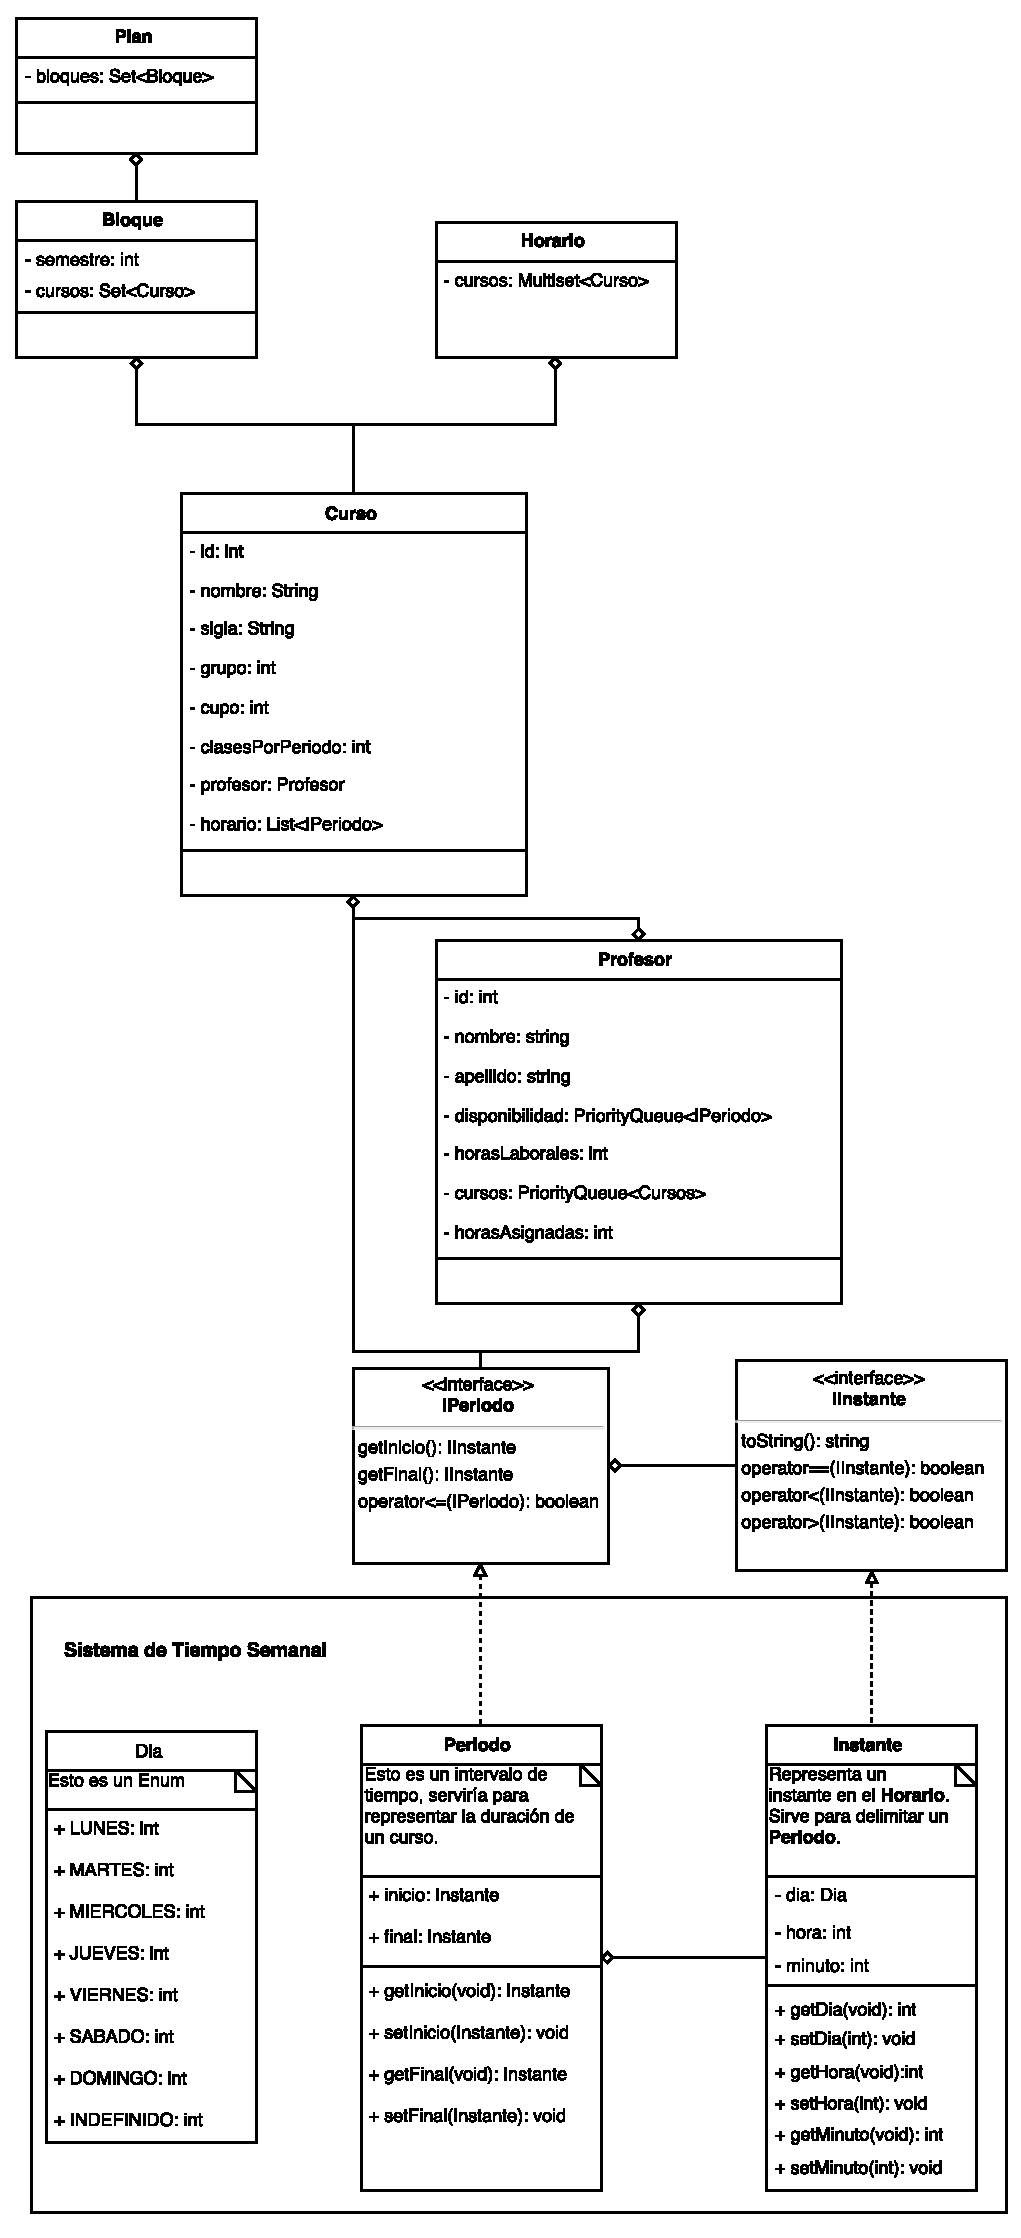
\includegraphics[trim={0 15.5cm 0 0}, clip]{HorariosCursos.pdf}
\newpage
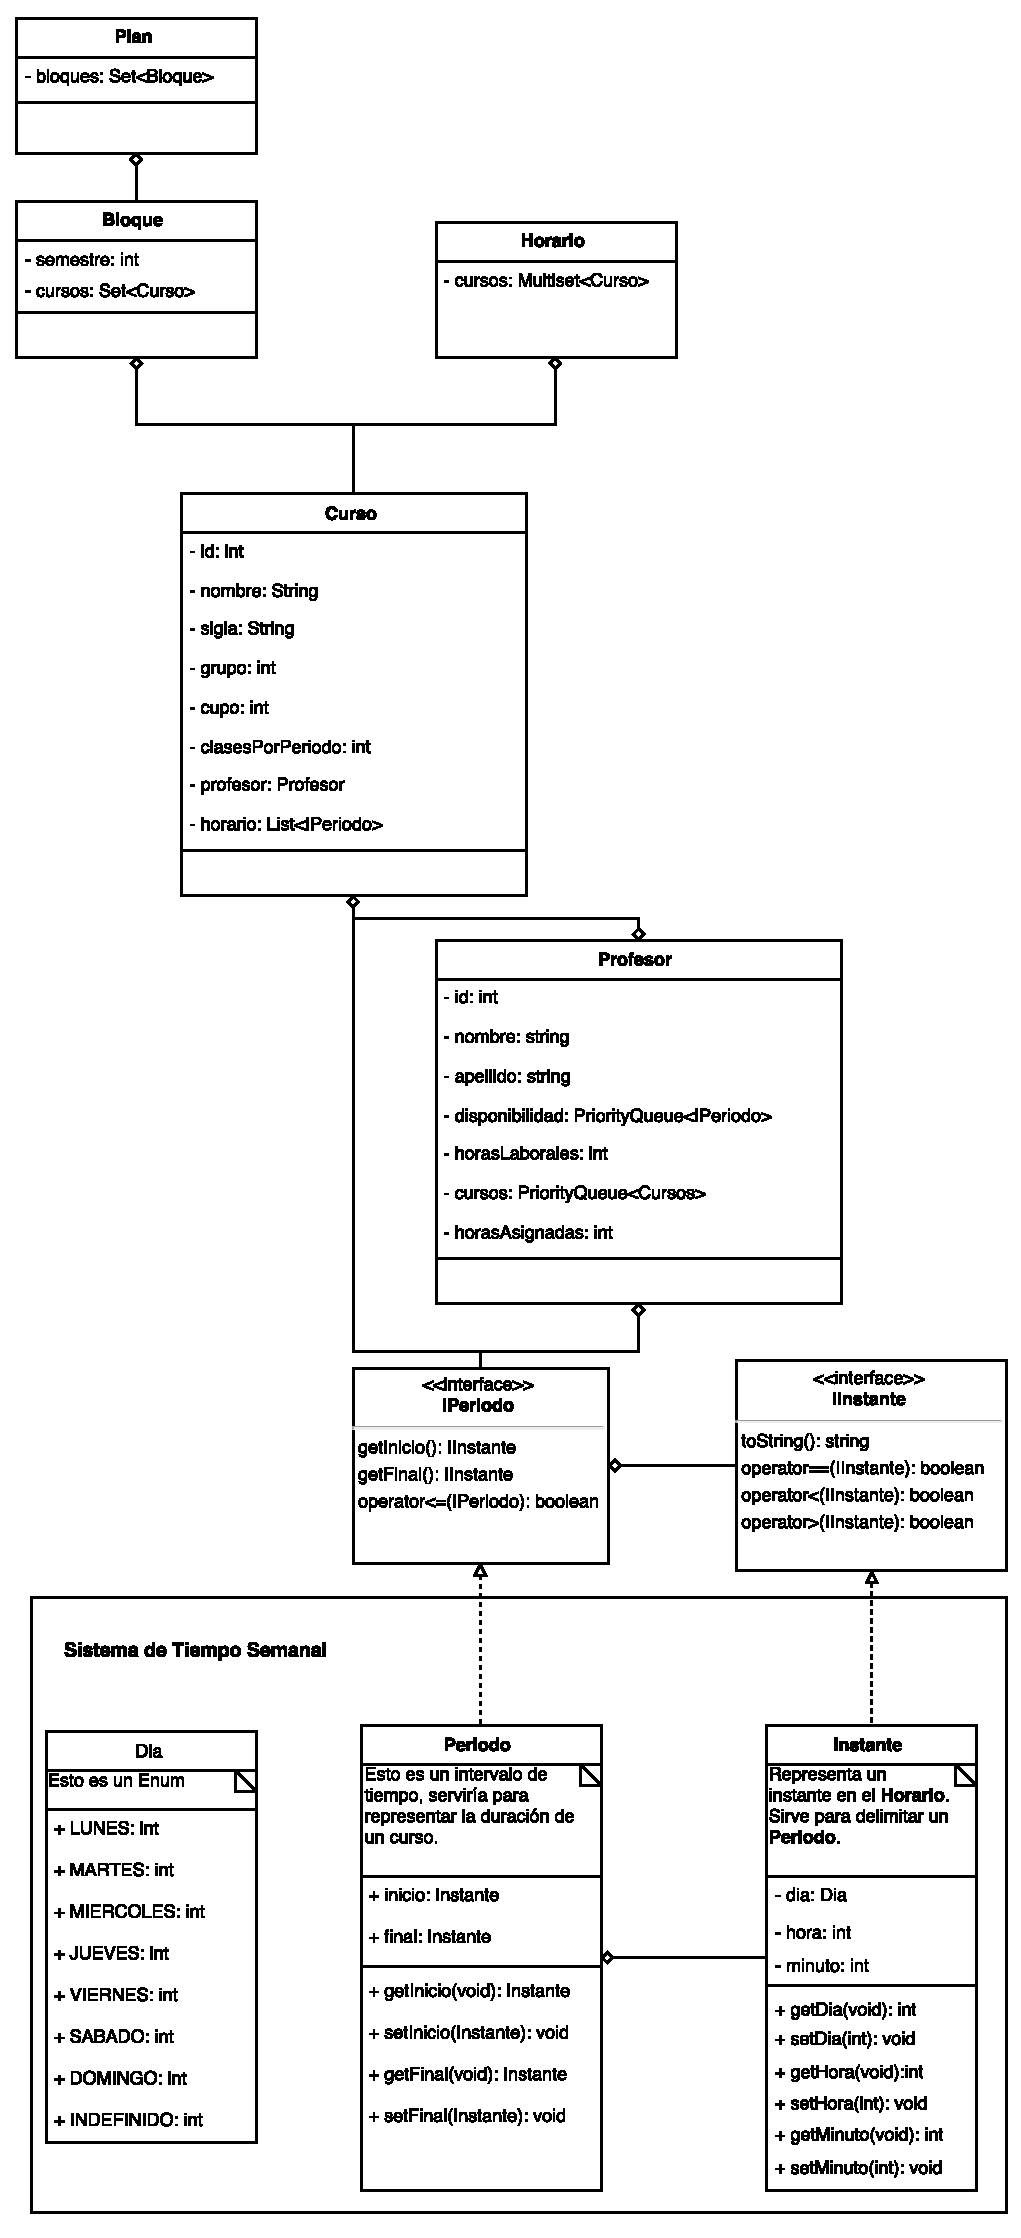
\includegraphics[trim={0 0 0 22.3cm}, clip]{HorariosCursos.pdf}
\begin{center}
	\textit{Diagrama de clases}
\end{center}

El diagrama anterior muestra las principales clases e interfaces que se
utilizaran para el desarrollo de la aplicación. La mayoría de las clases aún
no cuentan con métodos, esto se agregara en etapas posteriores del desarrollo.
Se muestran, sin embargo, los atributos de todas las clases, los cuales, se
pretende mantener a menos que surga la necesidad de añadir o eliminar atributos.
\newpage
\end{document}
